% This was adapted from https://github.com/deselaers/latex-beamerposter/blob/master/examples/03/poster.tex
%
% POSTER DRAFT v4 (20/10/2026) -- DML 2026.
% Layout (v4, 20/10): left = problem (+ typical sample), Mamba (+ fig_block),
% finding 1, references; right = findings 2-4 (4 with the separated-flow
% sample), take-home. "How we measured"
% removed (report material); its two facts the poster needs are in block 2.
% The preamble of the course template (class, packages, theme, fonts) is
% UNCHANGED. Only the content is new: title, authors, blocks.
% - Figures: docs/figures/poster/ of the repo, copied to img/. They are
%   included at \linewidth; the layout (v4) was checked with these sizes
%   (width x height): left column fig_sample 16.2 x 4.2, fig_block
%   16.2 x 6.0; right column fig_level 22.4 x 6.0, fig_ablation 22.4 x 8.0,
%   fig_tail_val 22.4 x 4.5 cm. Body text 16 pt, captions 9.4 pt.
%   With taller figures the left column overflows (it is at its limit).
% - Numbers: TEST = pre-registered, official test set; VAL = exploratory,
%   validation set. Source: docs/lab-notebook.md and the CSVs behind the
%   figures (scripts/poster_figures.py).
% - bib.bib = a copy of the report's references.bib + extra_refs.bib
%   (yu2025mambaout, he2019mgnet).
% - The full-data-set experiment is NOT on the poster (decided 18-19/10).


\documentclass{beamer}
\usepackage[orientation=portrait,size=a2,scale=1.3,debug]{beamerposter}
\mode<presentation>{\usetheme{ZH}}
\usepackage{chemformula}
\usepackage[utf8]{inputenc}
\usepackage[german, english]{babel} % required for rendering German special characters
\usepackage{siunitx} %pretty measurement unit rendering
\usepackage{hyperref} %enable hyperlink for urls
\usepackage{ragged2e}
\usepackage[font=footnotesize,justification=justified]{caption}
\usepackage{array,booktabs,tabularx}
\usepackage{lipsum}
\usepackage{blindtext}
\usepackage{qrcode}

% Replacement font for Akzidenz
\usepackage{helvet}

\usepackage{beamerthemeZH} 

% 1. DEFINIZIONE DELLA NUOVA PALETTE
\definecolor{ChalmersBlue}{RGB}{0, 43, 73}      % Blu principale (intestazioni)
\definecolor{ChalmersAccent}{RGB}{217, 83, 30}   % Arancione (per far risaltare il testo)
\definecolor{Bordeaux}{RGB}{160, 18, 40}
\definecolor{ta2gray}{RGB}{204, 204, 204}

\newcolumntype{Z}{>{\centering\arraybackslash}X} % centered tabularx columns
%\sisetup{per=frac,fraction=sfrac}

% ---- draft helper (content only, no style change): figure placeholder ----
% \placeholder{description}{height}
\newcommand{\placeholder}[2]{\fbox{\parbox[c][#2][c]{0.93\linewidth}{\centering
  \textbf{PLACEHOLDER}\\[4pt]#1}}}
% -------------------------------------------------------------------------

% Where does Mamba help a U-Net \\ predicting airfoil flows?
\title{\huge Airfoil Flow Prediction: \textit{Where} and \textit{Why} Mamba Blocks Enhance U-Net Architectures}
\author{\textbf{Group 62}: Cristiano Corona, Francesca Marina Pozzi}
\institute[Chalmers]{Chalmers University of Technology \\ Electrical Engineering Department}
\date{October 27, 2026}

% edit this depending on how tall your header is.
\newlength{\columnheight}
\setlength{\columnheight}{50cm}


\begin{document}
\begin{frame}
\begin{columns}
	% =================================================================
	% LEFT COLUMN: problem, Mamba, finding 1, references
	% =================================================================
	\begin{column}{.48\textwidth}
		\begin{beamercolorbox}[center]{postercolumn}
			\begin{minipage}{.98\textwidth}  % tweaks the width, makes a new \textwidth
				\parbox[t][\columnheight]{\textwidth}{
					\begin{myblock}{Problem: a fast surrogate for RANS}
						\begin{itemize}
							\item CFD is \emph{too slow} for design loops. A \textbf{\textcolor{Bordeaux}{U-Net}} (DfpNet, 2.3\,M params) maps free stream and airfoil mask ($128\times128$) to $p$, $v_x$, $v_y$ in one forward pass \cite{thuerey2020}. Pressure obeys a Poisson equation: every point depends on the whole domain.
						\end{itemize}
						\begin{equation*}
							\nabla^2 P = -\rho\,\partial_i\partial_j\big(U_iU_j+\overline{u'_iu'_j}\big)
						\end{equation*}
                        \vspace{-0.7cm}
						\begin{figure}
							\centering
                            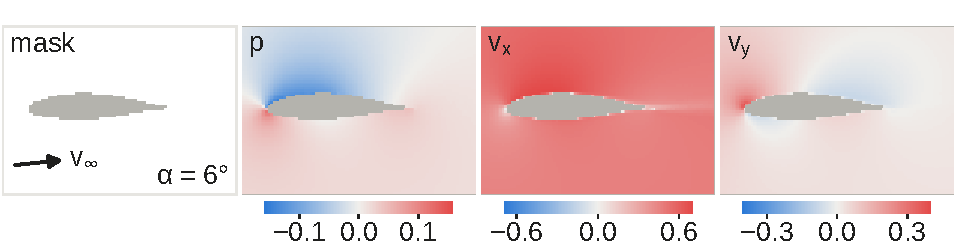
\includegraphics[width=\linewidth]{img/fig_sample.pdf}
							
							\caption{One validation sample: $v_x$ is mostly free stream, $v_y$ is induced by the airfoil.}
						\end{figure}
						\textbf{Question}: convs are local. Does a \emph{global} block help, and \emph{where}? 						
                        
                        \textbf{Expected}: the largest gain on $p$.
					\end{myblock}\vfill
					\begin{myblock}{Mamba instead of attention}
						\begin{itemize}
							\item \textbf{\textcolor{Bordeaux}{Attention}}:  every pixel with every pixel, cost $O(L^2)$ in the $L$ tokens \cite{vaswani2017}.
							\item \textbf{\textcolor{Bordeaux}{Mamba}}: a \emph{selective state space model} scanned along the image in 4 directions (SS2D), cost $O(L)$ \cite{gu2024mamba,liu2024vmamba}.
						\end{itemize}
						
						\begin{figure}
							\centering
							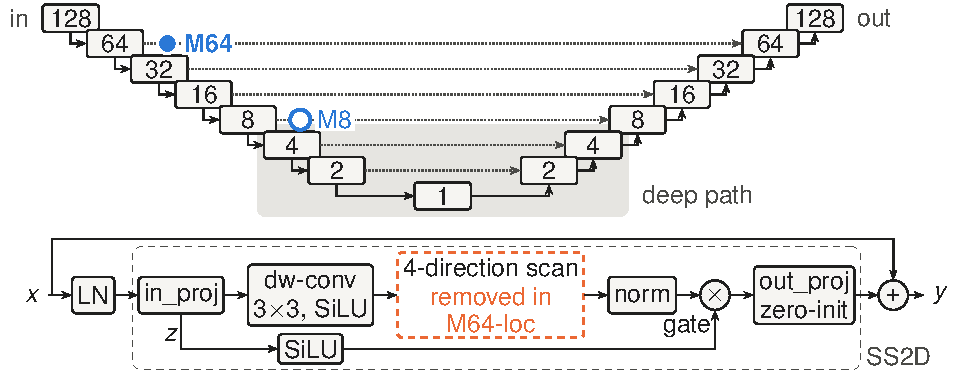
\includegraphics[width=\linewidth]{img/fig_block.pdf}
							%\caption{Top: DfpNet and the two insertion points. Bottom: the residual Mamba (SS2D) block. Its output projection starts at zero, so at initialisation the network \emph{is} the baseline.}
                            \caption{Top: DfpNet and insertion points. Bottom: residual Mamba (SS2D) block, zero-initialised: at the start the network \emph{is} the baseline.}
                            \vspace{-0.8cm}
						\end{figure}
					\end{myblock}\vfill
					\begin{myblock}{1. Deep levels: Mamba adds nothing, but can replace them}
						\begin{itemize}
							\item A Mamba block at $8\times8$: no test gain ($-0.01$ [$-0.34$, $+0.26$]); it fits training data better, not new shapes.
							\item \textbf{Why}: the \textbf{\textcolor{Bordeaux}{deep path}} below $8\times8$ (79\% of the weights) already has a \emph{global receptive field}.
						\end{itemize}
						\vspace{0.4cm}
                        \begin{center}
                        \begin{tabular}{l l @{\hspace{1.5cm}} c}
                            \toprule
                            & Deep path & Test error (5 seeds) \\
                            \midrule
                            U-Net & convolutions down to $1\times1$ & 2.90\% \\
                            Truncated & removed & 3.47\% \\
                            \textbf{Mamba} & \textbf{11 Mamba blocks at $\boldsymbol{8\times8}$} & \textbf{2.79\%} \\
                            \bottomrule
                        \end{tabular}
                        \end{center}
						\vspace{0.3cm}
						Replacing the deep path with Mamba blocks \emph{lowers the error} by $0.69$ points \textit{vs.} Truncated (95\% CI = $[0.26,\,1.10]$), and matches the U-Net.
					\end{myblock}\vfill
					\begin{myblock}{References}
						\footnotesize
						\bibliographystyle{abbrv}
						\bibliography{poster-template/bib} 
					\end{myblock}\vfill
		}\end{minipage}\end{beamercolorbox}
	\end{column}
	% =================================================================
	% RIGHT COLUMN: findings 2-4 + take-home
	% =================================================================
	\begin{column}{.52\textwidth}
		\begin{beamercolorbox}[center]{postercolumn}
			\begin{minipage}{.98\textwidth} % tweaks the width, makes a new \textwidth
				\parbox[t][\columnheight]{\textwidth}{
					\begin{myblock}{2. At $64\times64$: $v_y$ error $-18\%$ on the test set}
						\begin{figure}
							\centering
							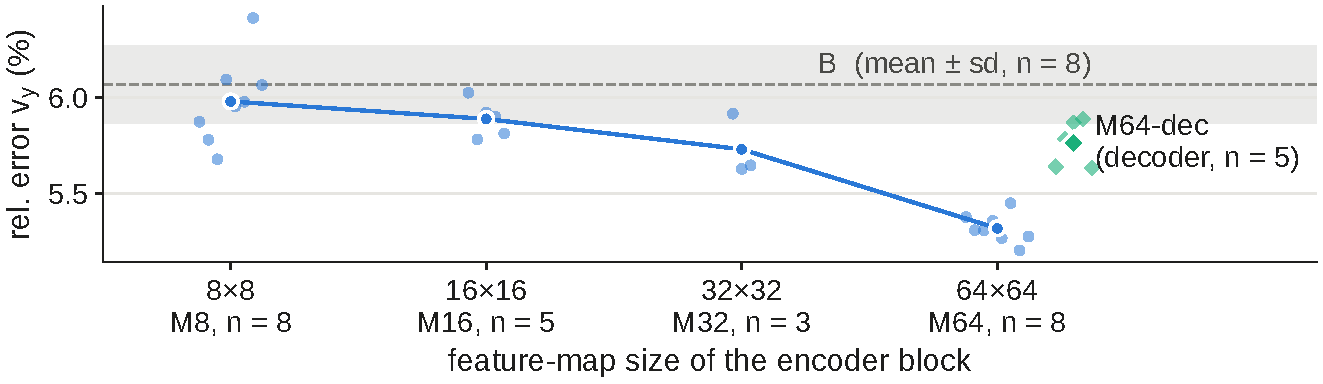
\includegraphics[width=\linewidth]{img/fig_level.pdf}
							\caption{Validation $v_y$ error \textit{vs.} encoder block resolution (M8\,--\,M64). Dots: seeds; large dot: mean; grey band: baseline B, mean $\pm$ s.d. The same block in the decoder (M64-dec) helps less.}
						\end{figure}
						\begin{itemize}
							%\item At $64\times64$ the U-Net applies a single convolution: it barely processes the field.
							%\item Pre-registered test on unseen airfoils (opened after exploring on validation): $v_y$ error $6.64\% \rightarrow 5.47\%$ ($-1.17$ [$-2.47$, $-0.43$]), \textbf{confirmed}. $p$ and combined error ($\approx v_x$ error): no demonstrated difference.
                            \item \textbf{Why $\boldsymbol{64\times64}$}: here the U-Net applies a single conv.,
                            so the field is barely processed $\rightarrow$ the gain grows with resolution.
                            \item \textbf{Confirmed on unseen airfoils} (pre-registered, 30 unseen profiles, 3 flows per profile): $-1.17$ points on $v_y$ error (95\% CI = $[-2.47,\,-0.43]$).
                            \item \textbf{No demonstrated difference} on $p$, $v_x$ and combined error ($0\in$ 95\% CI).
						\end{itemize}
					\end{myblock}\vfill
					\begin{myblock}{3. Ablation: the gain does not need the SSM}
						\begin{figure}
							\centering
							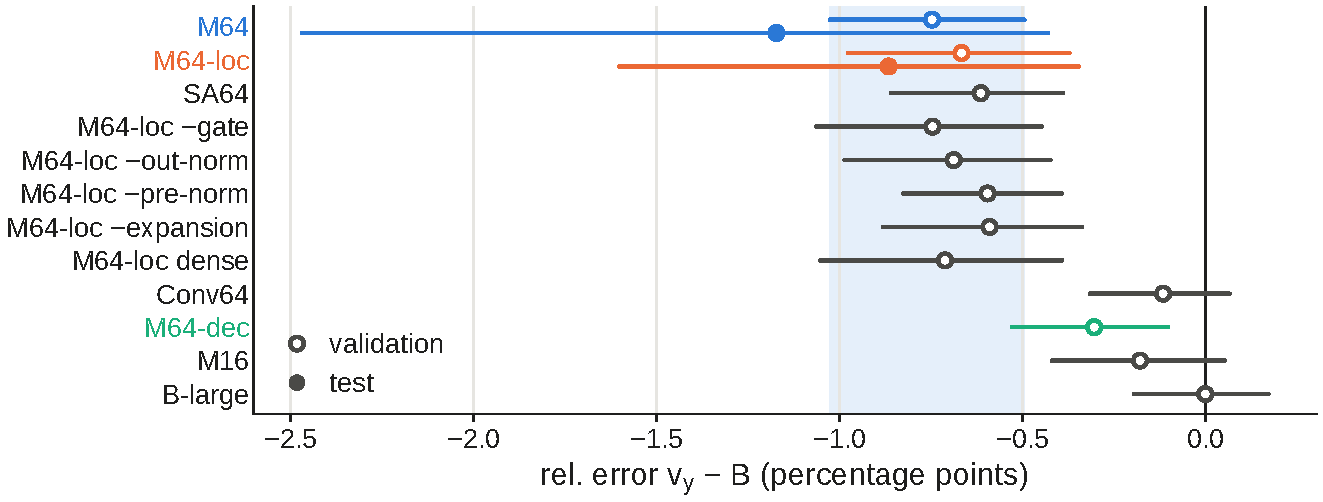
\includegraphics[width=\linewidth]{img/fig_ablation.pdf}
							\caption{Difference in $v_y$ error to the baseline, 95\% two-level bootstrap intervals. Open: validation (8 seeds for M64, M64-loc, B-large; 5 for the others); filled: pre-registered test. Band: validation interval of M64.}
						\end{figure}
						\begin{itemize}
							%\item \textbf{Scan removed} (M64-loc): most of the gain stays. \textbf{Attention} (SA64) gives it too, at $16\times$ the training time. \textbf{A plain conv block} (Conv64) does not.
							%\item \textbf{Final architecture:} U-Net + M64-loc (+7\,k parameters, $1.6\times$ training time). Test: $-0.87$ [$-1.60$, $-0.35$] points ($-13\%$), \textbf{confirmed}. Consistent with MambaOut \cite{yu2025mambaout}.
                            \item \textcolor{Bordeaux}{No scan} (M64-loc): most of the gain stays. \textcolor{Bordeaux}{Attention} (SA64) matches it, but trains $17\times$ slower than B. \textcolor{Bordeaux}{A plain conv. block} (Conv64) gives no proven gain.
                            \item \textbf{Final architecture}: \textbf{\textcolor{Bordeaux}{U-Net + M64-loc}} ($+7$\,k parameters, $1.6\times$ training time vs.\ B). Test: $-0.87$ $[-1.60,\,-0.35]$, \textbf{confirmed}. \newline Consistent with MambaOut \cite{yu2025mambaout}.
                            \item \textbf{Full 53.8k set} (validation, 3 seeds): M64-loc retains a smaller $v_y$ gain ($-0.22$ points, $-4.7\%$ vs.\ B); wall-band $v_y$ MAE is $6.1\%$ lower.
						\end{itemize}
					\end{myblock}\vfill
					\begin{myblock}{4. Expected on $p$, found on $v_y$: why?}
						%\textit{Our reading, consistent with the data but not tested directly.}
						%\begin{itemize}
							%\item \textbf{The global part of $p$ is already solved:} it is smooth, and a U-Net is shaped like a multigrid V-cycle, the classic Poisson solver \cite{he2019mgnet}.
							%\item \textbf{The $p$ error lives in a tail}: separated flows at high angle, missed by \emph{every} model we checked (2.5\% of the samples carry $\sim$15\% of the error; figure). Test: the mean $p$ error drops ($-1.8$ [$-5.4$, $+0.1$]), the median sample does not ($-0.01$ [$-1.4$, $+0.9$]).
							%\item \textbf{The gain is local, at the wall}: wall-band $v_y$ error $-11\%$, no scan needed. $v_y$ is almost all airfoil-induced (Fig.~1), so a near-wall gain shows on $v_y$; on $v_x$ the free stream dilutes it.
						%\end{itemize}
                        \textit{Our reading: consistent with the data, not tested directly.}
                        \begin{itemize}
                        	\item \textbf{The global part of $p$ is already solved}: $p$ is smooth, and a U-Net works like a multigrid V-cycle, the classic Poisson solver \cite{he2019mgnet}.
                        	\item \textbf{The $p$ error sits in a tail of hard cases}: separated flows at high angle, missed by all models (2.5\% of samples carry $\sim$15\% of the error). Test: no demonstrated change in $p$ error with M64 (mean $-1.8$ [$-5.4$, $+0.1$]).
                        	\item \textbf{The gain is local, at the wall}: within 4 px of the airfoil, $v_y$ error drops by $11\%$ (M64) and $10\%$ without the scan (M64-loc) $\rightarrow$ $v_y$ is almost entirely \emph{airfoil-induced} (Fig.~1), so the gain shows on $v_y$ but not on $v_x$.
                        \end{itemize}
                                            \vspace{0.3cm}
											\begin{figure}
                                            
							\centering
							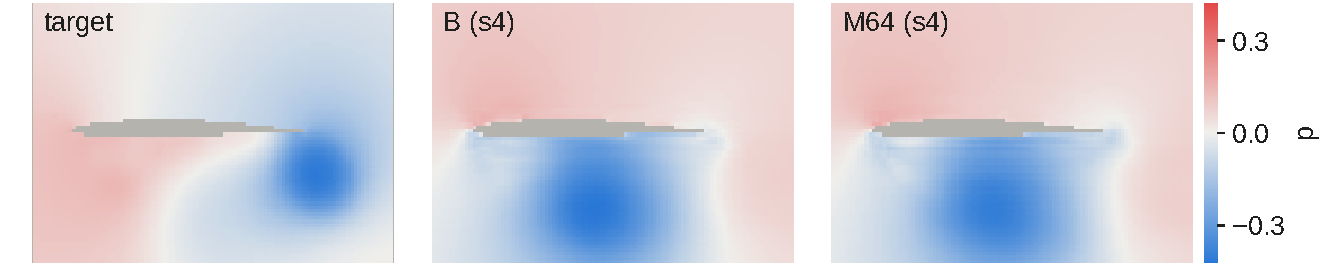
\includegraphics[width=\linewidth]{img/fig_tail_val.pdf}
							\caption{Pressure on a separated validation flow at $-22^\circ$: the target sheds a vortex behind the airfoil; B and M64 keep it attached.}
						\end{figure}
					\end{myblock}\vfill
					\begin{myblock}{Take-home}
                        \begin{minipage}[c]{0.72\linewidth}
                            \begin{itemize}
                                \item The U-Net already handles the global, elliptic part; it lacks processing at \textbf{high resolution}.
                                \item There a \textbf{\textcolor{Bordeaux}{gated Mamba-style block}} cuts the $v_y$ error by 13--18\%; most of the gain remains \textbf{without the SSM}. With $8\times$ more data, the gain roughly halves.
                            \end{itemize}
                        \end{minipage}\hfill
                        \begin{minipage}[c]{0.20\linewidth}
                            \centering
                            \color{black}
                            \qrcode[height=2.6cm]{https://github.com/CristianoCorona/MambaDeepFlow}\\[4pt]
                            {\scriptsize \textbf{Project Repository}}
                        \end{minipage}
                    \end{myblock}\vfill
		}\end{minipage}\end{beamercolorbox}
	\end{column}
\end{columns}
\end{frame}
\end{document}





